%----------------------------------------------------------------------------
\chapter{Optimalizációs megközelítések}
\label{sec:optimalizacios-megkozelitesek}

A mérnököktől nap mint nap problémák megoldását várják el. A probléma megjelenésétől a felismerésén át, a megoldás megtalálásáig és megvalósításáig számos kisebb és nagyobb feladat vár elkészítésre. Ezt a folyamatot a sztochasztikus modellek paramétereinek optimalizálása esetében a \ref{fig:folyamat}. ábra szemlélteti.

\begin{figure}[!ht]
	\centering
	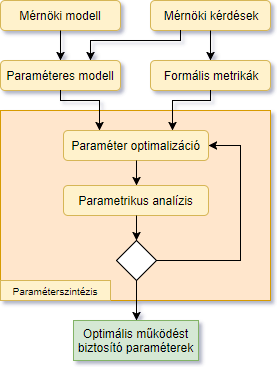
\includegraphics[width=90mm, keepaspectratio]{figures/optmeg.png}
	\caption{Paraméter optimalizálás folyamata}
	\label{fig:folyamat}
\end{figure}

Egy modellben összefoglalhatjuk az összes jelentékeny tényezőjét a feladatnak. Kapcsolatokat definiálhatunk állapotok között, eseményeket köthetünk hozzájuk, úgy általában magunk előtt láthatjuk általa a rendszer viselkedését. Jó példa erre a \textbf{Petri háló}val való modellezés. A Petri hálók tökéletesen alkalmasak információs folyamatrendszerek leírására és tanulmányozására, akár aszinkron, párhuzamos, nem-determinisztikus vagy sztochasztikus rendszerek esetén. Grafikus és matematikai eszköz is egyben, így lehetővé teszi számunkra, hogy matematikai viselkedéssel ruházzuk fel a rendszerünket, egyenlőségekkel, egyenletekkel, valószínűségekkel, paraméterekkel.\cite{PetriCikk}

Tulajdonképpen egy irányított gráfot definiálunk, melyben az \textbf{irányított élek} \textbf{hely}eket és \textbf{átmenet}eket kötnek össze. Minden helyen tetszőleges számban lehetnek ``\textbf{token}ek'', melyek a folyamat nyomon követését teszik szemléletesebbé. Ha egy átmenetnél teljesülnek a \textbf{tüzelési feltétel}ek, az átmenet tüzel, és a bemenő helyeken lévő adott számú tokent a kimeneti helyek tokenjeivé ``alakítja át''.

A rendszer ilyen szintű megismerése után fontos mérföldköve a tervezésnek olyan kérdések keresése és feltevése, melyek kulcsfontosságúak lehetnek a rendszer működésében. Mikor következik be? Mik hatnak egymásra? Milyen kapcsolat van közöttük? Hogyan befolyásolja a folyamatot? A jó kérdések feltevése nem könnyű, de elengedhetetlen ahhoz, hogy újabb lépéseket tudjunk tenni a célunk felé.

A kérdések tulajdonképpen informális megfogalmazásai olyan matematikai összefüggéseknek, melyek a rendszerünk viselkedését befolyásolják. Ezek a \textbf{reward függvény}ek olyan metrikákat írnak le, melyek kimenete mérhető. 

Ritka eset az, amikor teljes körű ismerettel rendelkezünk egy probléma minden részletéről. A legtöbb esetben elhanyagoljuk, vagy ismeretlen változóként a modellben hagyjuk azokat a részleteket, tulajdonságokat, értékeket, amelyekről nincs tudomásunk. 
Sztochasztikus modell esetén valószínűségi eloszlásokról, várható értékekről, tüzelési valószínűségekről, rátákról beszélünk. Példáinkban a tüzelési valószínűségek exponenciális eloszlást követnek. Az exponenciális eloszlás rátája, $\lambda$
függhet a modell paramétereitől. Ezáltal befolyásolják a hatótényezők a rendszert. Konkrét példákat ilyen modellekre \aref{sec:fuggelek}. függelékben mutatok be.

A metrikáink függenek ezektől a \textbf{paraméter}ektől, azonban ennek a függésnek az alakját, tulajdonságait nem ismerjük. Ahhoz, hogy megtaláljuk egy sokdimenziós modell esetén azt az optimális paraméterlekötést, mellyel a rendszer teljesíti a követelményeket, paraméterszintézis során alkalmazunk különböző optimalizáló algoritmusokat.

A szintézis minden iterációjában újabb és újabb paraméterekkel futtatjuk le az analízist, majd az adott algoritmus működése alapján műveleteket végzünk a kapott eredményen, mely alapján eldönthetjük, elértük-e a leállási feltételt, és ha nem, az értelmezési tartomány mely pontjának a kiértékelése visz minket a legnagyobb valószínűséggel közelebb az optimális ponthoz. Ez lesz az a pont, amellyel a szintézis következő iterációjában folytatjuk a műveleteket.

A \textbf{célfüggvény}, melyet optimalizálunk, sokféleképpen definiálható. Mi \aref({eq:celfgv}) képlettel leírt összes négyzetes hibát választottuk, mely egy azon megközelítések közül, mellyel általánosan leírható egy rendszer elvárt viselkedéstől való eltérése.

\section{Algoritmusok használhatóságának szempontjai}

A paraméter optimalizálás során azt a pontot keressük, mely a rendszer hibáját nullára csökkenti. Ennek az elérését azonban számos tényező nehezíti, mind a tervező, mind az algoritmusok szempontjából.

Az \textbf{analízist végző keretrendszer költséges}en skálázódik a paraméterek dimenziójának növekedésével. Célunk egy olyan optimalizáló használata, mely ezt a költséget -- mely a mi esetünkben főleg a futási időt jelenti -- is minimalizálja.

Lehetőségünk van nemcsak függvényérték, de az egyes paraméterek szerinti érzékenység, vagyis parciális derivált kiszámítására is. Ennek köszönhetően szóba jöhetnek azok az ismert algoritmusok is, melyek egyszer, vagy többször differenciálható célfüggvényt feltételeznek. Tisztában kell lennünk azonban azzal, hogy ezért drága árat fizetünk, hisz a mi célfüggvényünk esetében (\ref{eq:celfgv}) egy \textbf{gradiens számítás} $O(n)$ számítást jelent, egy Hesse-mátrix $O(n^2)$ költséget jelentene, ahol a célfüggvény $j.$ paramétere szerinti parciális deriválja
$$\frac{\partial f}{\partial p_j}=\sum_{i=1}^{rewards}\left\lbrace   2\cdot \left( \hat{R}_i-R_i\right) \cdot\left(-\frac{\partial R_i}{\partial p_j}\right)  \right\rbrace   .$$
Ezért a Hesse-mátrixszal számoló algoritmusok nem megfelelőek az elvárásainknak.

Az optimalizálás nagyon összetett feladat, különböző függvényekből pedig végtelen sok van. Nyilvánvaló, hogy egyetlen algoritmus képtelen mindegyikre jó megoldást találni. Elvárható azonban, hogy egy adott algoritmus ne csak egyetlen függvénytípus optimalizálására specializálódjon. Ezt az algoritmusok különböző típusú \textbf{hiperparaméter}ei teszik lehetővé, melyek beállítása a programozó felelőssége, és értékük nagy szerepet játszik az algoritmus pontosságában és hatékonyságában. Ezek megtalálása közel olyan nehéz, mint maga a modell optimumának a megtalálása. Az algoritmusokat megkülönbözteti ez is, hogy mekkora teret engednek a fejlesztőnek, mennyi és milyen megkötésekkel, változókkal, feltételezett modellekkel finomhangolható a működés. Minél jobban specializálható egy modellre az algoritmus, annál jobb eredményt érhetünk el az optimalizálás során.

Sztochasztikus, nemlineáris modelleket szeretnénk optimalizálni. Ezeknek a reward függvényeinek megvan az a sajnálatos tulajdonsága, hogy bizonyos \textbf{pontokban nem értelmezhetőek}. Ezen pontok ill. területek, akár csak maga a célfüggvény alakja, természetesen nem ismertek. Fekete doboz kényszerek mellett keressük a fekete doboz függvényünk globális minimumát. Elengedhetetlen tehát a hatékony működés érdekében, hogy -- jobb esetben -- elkerüljük az iterációk során ezen kiértékelhetetlen pontokat, vagy -- rosszabb esetben -- valamiképp kezelni tudjuk az algoritmus futása során ezen kiértékelhetetlen pontok számítására való igényt.

Összefoglalva, az alábbi szempontok alapján fogom vizsgálni a következő fejezetekben kipróbált optimalizáló algoritmusokat:

\begin{enumerate}
	\item Futási idő
	\item Deriváltak használatának szükségessége és eredményessége
	\item Hiperparaméterek mennyisége, minősége
	\item Kényszerek implementálhatósága
	\item Iterációk során kiszámítható és nem kiszámítható pontok aránya
\end{enumerate}